\section*{\large{ВВЕДЕНИЕ}}

Цель лабораторной работы --- реализовать программу шифрования симметричным алгоритмом \texttt{DES}~\cite{des} с применением \texttt{PCBC}~\cite{pcbc} режима шифрования.

Задачи лабораторной работы:

\begin{enumerate}
    \item провести анализ симметричного алгоритма шифрования \texttt{DES} и \texttt{PCBC} режима шифрования;
    \item описать вышеперечисленные алгоритмы;
    \item релизовать програмное обеспечение с использованием описанных алгоритмов.
\end{enumerate}

\clearpage
\section{Аналитическая часть}

\subsection{DES}

\texttt{DES} --- это блочный шифр, означающий, что он оперирует блоками открытого текста заданного размера (64 бита) и возвращает блоки зашифрованного текста того же размера. 
Таким образом, DES приводит к перестановке среди $2^{64}$ возможных расположений 64-х бит, каждое из которых может быть либо 0, либо 1. 
Каждый блок из 64 бит делится на два блока по 32 бита каждый, левая половина блока $\texttt{L}$ и правая половина $\texttt{R}$.

Пример: Пусть $\texttt{M}$ --- обычное текстовое сообщение 

$\texttt{M} = 0123456789ABCDEF$, 

где $\texttt{M}$ находится в шестнадцатеричном формате (основание 16). 

Переписав $\texttt{M}$ в двоичном формате, мы получим 64-битный блок текста:

\texttt{M} = 0000\ 0001\ 0010\ 0011\ 0100\ 0101\ 0110\ 0111\
         1000\ 1001\ 1010\ 1011\ 1100\ 1101\ 1110\ 1111

$\texttt{L} = 0000\ 0001\ 0010\ 0011\ 0100\ 0101\ 0110\ 0111$

$\texttt{R} = 1000\ 1001\ 1010\ 1011\ 1100\ 1101\ 1110\ 1111$

Первый бит \texttt{M} равен <<0>>. Последний бит равен <<1>>.

\texttt{DES} работает с 64-битными блоками, используя ключи размером 56 бит. 
Ключи фактически хранятся как имеющие длину 64 бита, но каждый 8-й бит в ключе не используется (т.е. биты под номерами 8, 16, 24, 32, 40, 48, 56, и 64). 

Пример: Пусть \texttt{K} --- шестнадцатеричный ключ:

$\texttt{K} = 133457799BBCDFF1$.

Это результирует в качестве двоичного ключа (устанавливая 1 = 0001, 3 = 0011 и т.д. и группируя вместе каждые восемь битов, из которых последний в каждой группе будет неиспользуемым):

\texttt{K} = 00010011\ 00110100\ 01010111\ 01111001\ 10011011\ 10111100\ 11011111\ 11110001

Алгоритм DES использует следующие шаги:

\subsubsection{Шаг 1: Создание ключей}

64-разрядный ключ переставляется в соответствии со следующей таблицей, PC-1, приведенная как таблица~\ref{tbl:pc-1}. 
Поскольку первая запись в таблице равна <<57>>, это означает, что 57-й бит исходного ключа K становится первым битом переставленного ключа K+,
49-й бит исходного ключа становится вторым битом переставленного ключа,
4-й бит исходного ключа является последним битом переставленного ключа и т.д.

\begin{table}[ht!]
    \begin{center}
		\captionsetup{justification=raggedright,singlelinecheck=off}
		\caption{\label{tbl:pc-1} PC-1}
        \begin{tabular}{ |c c c c c c c|}
                57 &   49  &  41  & 33   & 25  &  17  &  9 \\
                       1  & 58  &  50 &  42 &   34 &   26 &  18 \\
                      10 &   2 &   59 &  51 &   43 &   35 &  27 \\
                      19 &  11 &    3 &  60  &  52  &  44   & 36 \\
                      63  & 55 &   47  & 39  &  31  &  23  & 15 \\
                       7  & 62  &  54  & 46  &  38  &  30  & 22 \\
                      14  &  6  &  61  & 53  &  45  &  37  & 29 \\
                      21  & 13   &  5  & 28  &  20  &  12  &  4
        \end{tabular}
    \end{center}
\end{table}

Пример: Из исходного 64-разрядного ключа

$\texttt{K}$ = 00010011 00110100 01010111 01111001 10011011 10111100 11011111 11110001

получается 56-битную перестановку

$\texttt{K}^{+}$ = 1111000 0110011 0010101 0101111 0101010 1011001 1001111 0001111

Затем этот ключ разделяется на левую и правую половины, $C_0$ и $D_0$, где каждая половина содержит 28 бит.

Пример: Из переставленного ключа $\texttt{K}^{+}$ мы получаем

$C_0$ = 1111000 0110011 0010101 0101111

$D_0$ = 0101010 1011001 1001111 0001111

Определив $C_0$ и $D_0$, создаются шестнадцать блоков $C_n$ и $D_n$, $1<=n<=16$. 
Каждая пара блоков $C_n$ и $D_n$ формируется из предыдущей пары $C_{n-1}$ и $D_{n-1}$, соответственно, для n = 1, 2, ..., 16, используя следующий схеме <<сдвигов влево>> предыдущего блока. 
Чтобы выполнить сдвиг влево, перемещается каждый бит на одно место влево, за исключением первого бита, который циклически перемещается до конца блока.

\begin{table}[ht!]
    \begin{center}
		\captionsetup{justification=raggedright,singlelinecheck=off}
		\caption{\label{tbl:rot} Ротация битов}
        \begin{tabular}{ |c c| }
Iteration Number  &  Number of Left Shifts \\
                          1    &      1 \\
                          2     &     1 \\
                          3     &     2 \\
                          4     &     2 \\
                          5     &     2 \\
                          6     &     2 \\
                          7    &      2 \\
                          8     &     2 \\
                          9     &     1 \\
                         10     &     2 \\
                         11      &    2 \\
                         12     &     2 \\
                         13     &     2 \\
                         14    &      2 \\
                         15     &     2 \\
                         16      &    1
        \end{tabular}
    \end{center}
\end{table}

После этого формируются ключи $K_n$ для 1<=n<=16, применяя таблицу~\ref{tbl:pc-2} перестановок к каждой из сцепленных пар $C_n D_n$.
Каждая пара содержит 56 бит, но \texttt{PC-2} использует только 48 из них.

\begin{table}[ht!]
    \begin{center}
		\captionsetup{justification=raggedright,singlelinecheck=off}
		\caption{\label{tbl:pc-2} PC-2}
        \begin{tabular}{ |c c c c c c| }
                14 & 17 & 11 & 24 & 1 & 5 \\
3 & 28 & 15 & 6 & 21 & 10 \\
23 & 19 & 12 & 4 & 26 & 8 \\
16 & 7 & 27 & 20 & 13 & 2 \\
41 & 52 & 31 & 37 & 47 & 55 \\
30 & 40 & 51 & 45 & 33 & 48 \\
44 & 49 & 39 & 56 & 34 & 53 \\
46 & 42 & 50 & 36 & 29 & 32
        \end{tabular}
    \end{center}
\end{table}

Следовательно, первый бит $K_n$ является 14-м битом $C_n D_n$, второй бит - 17-м и так далее, заканчивая 48-м битом $K_n$, являющимся 32-м битом $C_n D_n$.

\subsubsection{Шаг 2: Кодировка 64-битных блоков}

Существует начальная перестановка IP, представленная в таблице~\ref{tbl:ip} из 64 бит данных сообщения M. 
Это переупорядочивает биты в соответствии со следующей таблицей, где записи в таблице показывают новое расположение битов по сравнению с их первоначальным порядком. 
58-й бит M становится первым битом IP, 50-й бит M становится вторым битом IP, и т.д. до 7-го бита M --- последнего бита IP.

\begin{table}[ht!]
    \begin{center}
	\captionsetup{justification=raggedright,singlelinecheck=off}
	\caption{\label{tbl:ip} IP}
        \begin{tabular}{ |c c c c c c c c|}
                58 &    50  & 42  &  34  &  26  & 18  &  10 &   2 \\
60  &  52  & 44  &  36  &  28  & 20  &  12   & 4 \\
62  &  54  & 46  &  38  &  30  & 22  &  14   & 6 \\
64  &  56  & 48  &  40  &  32  & 24  &  16   & 8 \\
57  &  49  & 41  &  33  &  25  & 17  &   9   & 1 \\
59  &  51  & 43  &  35  &  27  & 19  &  11   & 3 \\
61  &  53  & 45  &  37  &  29  & 21  &  13   & 5 \\
63  &  55   & 47 &   39  &  31  & 23  &  15  &  7
        \end{tabular}
    \end{center}
\end{table}

Пример: Применяя начальную перестановку к блоку текста M, приведенному ранее, получается следующее:

М = 0000 0001 0010 0011 0100 0101 0110 0111 1000 1001 1010 1011 1100 1101 1110 1111

IP = 1100 1100 0000 0000 1100 1100 1111 1111 1111 0000 1010 1010 1111 0000 1010 1010

Здесь 58-й бит M равен <<1>>, который становится первым битом IP. 50-й бит M равен <<1>>, который становится вторым битом IP. 7-й бит M равен <<0>>, который становится последним битом IP.

Затем перестановочный блок IP разделяется на левую половину $L_{0}$ из 32 бит и правую половину $R_0$ из 32 бит.

Пример: Из IP мы получаем $L_0$ и $R_0$

$L_0 = 1100 1100 0000 0000 1100 1100 1111 1111$

$R_0 = 1111 0000 1010 1010 1111 0000 1010 1010$

После этого выполняется 16 итераций для 1<=n<=16, используя функцию f, которая оперирует двумя блоками --- блоком данных из 32 бит и ключом Kn из 48 бит --- для получения блока из 32 бит. 
Пусть + обозначает сложение XOR, (побитовое сложение по модулю 2). 
Затем для n, идущих от 1 до 16, мы вычисляем:

$L_n = R_{n-1}$

$R_n = L_{n-1} + f(R_{n-1},K_{n})$

Это приводит к получению конечного блока, для n = 16, из $L_{16}\ R_{16}$. То есть, на каждой итерации мы берем правые 32 бита предыдущего результата и превращаем их в левые 32 бита текущего шага. Для правых 32 бит на текущем шаге мы выполняем XOR для левых 32 бит предыдущего шага с вычислением f .

Пример: Для n = 1 мы имеем

$K_1$ = 000110 110000 001011 101111 111111 000111 000001 110010

$L_1$ = $R_0$ = 1111 0000 1010 1010 1111 0000 1010 1010

$R_1 = L_0 + f(R_0,K_1)$

Чтобы вычислить $f(R_0,K_1)$, сначала расширяется каждый блок $R_{n-1}$ с 32 бит до 48 бит. 
Это делается с помощью таблицы выбора, которая повторяет некоторые биты в $R_{n-1}$. 
Данная таблица представлена как таблица~\ref{tbl:e} и будет именоваться как $E$. 
Таким образом, $E(R_{n-1})$ имеет 32-битный входной блок и 48-битный выходной блок.
Пусть $E$ таково, что 48 бит его выходных данных, записанных в виде 8 блоков по 6 бит в каждом, получены путем выбора битов на его входных данных по порядку в соответствии со следующей таблицей:

\begin{table}[ht!]
    \begin{center}
	\captionsetup{justification=raggedright,singlelinecheck=off}
	\caption{\label{tbl:e} E}
        \begin{tabular}{ |c c c c c c|}
                2  &   1   &  2   &   3   &   4   &  5 \\
                  4   &   5  &   6   &   7     & 8  &   9 \\
                  8    &  9   & 10    & 11   &  12   & 13 \\
                 12   &  13  &  14  &   15   &  16  &  17 \\
                 16   &  17  &  18  &   19   &  20  &  21 \\
                 20   &  21  &  22  &   23  &   24  &  25 \\
                 24   &  25  &  26  &   27  &   28  &  29 \\
                 28   &  29  &  30  &   31   &  32  &   1 \\
        \end{tabular}
    \end{center}
\end{table}

Таким образом, первые три бита $E(R_{n-1})$ являются битами в позициях 32, 1 и 2 $R_{n-1}$, в то время как последние 2 бита $E(R_{n-1})$ являются битами в позициях 32 и 1.

Пример: Вычисляется $E(R_0)$ из $R_0$ следующим образом:

$R_0$ = 1111 0000 1010 1010 1111 0000 1010 1010

$E(R_0)$ = 011110 100001 010101 010101 011110 100001 010101 010101

Далее в вычислении функции $f$ выполняется XOR для выходных данных $E(R_{n-1})$ с помощью ключа $K_n$:

$K_n + E(R_{n-1})$.

Пример: Для $K_1$, $E(R_0)$ имеется:

$K_1$ = 000110 110000 001011 101111 111111 000111 000001 110010

$E(R_0)$ = 011110 100001 010101 010101 011110 100001 010101 010101

$K_1+E(R_0)$ = 011000 010001 011110 111010 100001 100110 010100 100111.

Далее предыдущий результат, который равен 48 битам, записывается в виде:

$K_n + E(R_{n-1}) = B_1 B_2 B_3 B_4 B_5 B_6 B_7 B_8$,

где каждая $B_i$ представляет собой группу из шести битов. 

После этого вычисляется:

$S_1(B_1)S_2(B_2)S_3(B_3)S_4(B_4)S_5(B_5)S_6(B_6)S_7(B_7)S_8(B_8)$

где $S_i(B_i)$ относится к выходным данным $i$-го блока $S$.

Если $S_1$ --- это функция, определенная в этой таблице, а $B$ --- блок из 6 бит, то $S_1(B)$ определяется следующим образом: 

Первый и последний биты $B$ представляются как двоичное число в десятичном диапазоне от 0 до 3 (или двоичном от 00 до 11). 
Пусть этим числом будет $i$. 
Средние 4 бита $B$ представляют как двоичное число в десятичном диапазоне от 0 до 15 (двоичный код от 0000 до 1111). 
Пусть это число равно $j$. 
В таблице находится число в $i$-й строке и $j$-м столбце. 
Это число в диапазоне от 0 до 15 и однозначно представлено 4-битным блоком. 
Этот блок является выходом $S_1(B)$ из $S_1$ для входного блока $B$. 
Например, для входного блока $B = 011011$ первый бит равен <<0>>, а последний бит <<1>> дает 01 в качестве строки. 
Это строка 1. 
Средние четыре бита - это <<1101>>. 
Это двоичный эквивалент десятичного числа 13, поэтому столбец имеет номер 13. 
В строке 1 и столбце 13 помещено число 5, что и определяет выходные данные; 5 --- двоичное значение которого равно 0101 --- следовательно, $S_1(011011) = 0101$.
Таблицы для определения $S_1 ... S_8$ показаны на рисунке~\ref{fig:des-tables}:

\begin{figure}[ht!]
	\centering
	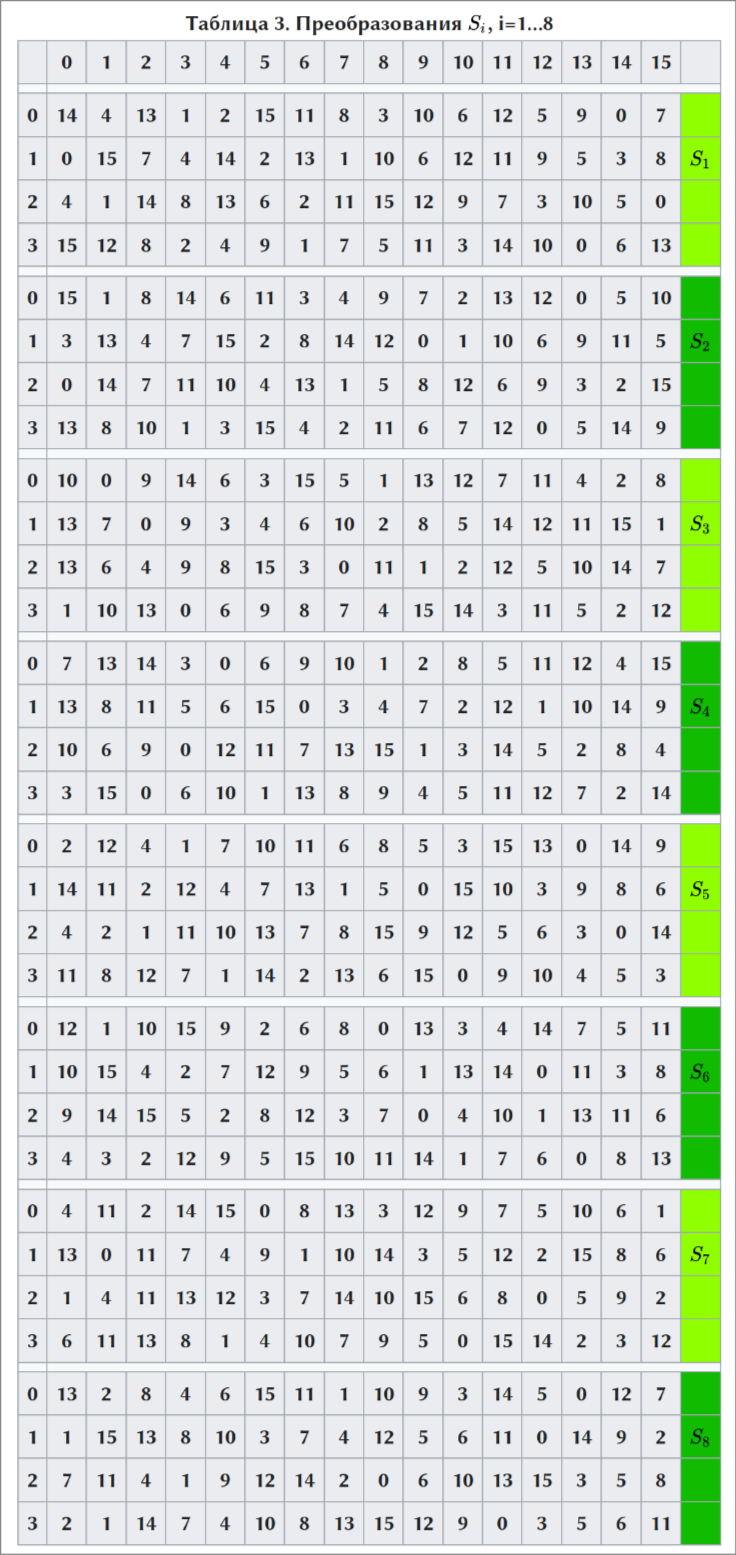
\includegraphics[width=0.65\linewidth]{assets/images/des-tables.png}
	\caption{Таблицы $S_1 ... S_8$}
	\label{fig:des-tables}
\end{figure}
\clearpage

Заключительным этапом вычисления функции $f$ является выполнение перестановки $P$ выходных данных для получения конечного значения функции $f$:

$f = P(S_1(B_1)S_2(B_2) ... S_8(B_8))$

Перестановка $P$ определена таблице~\ref{tbl:p}.
$P$ выдает 32-разрядный выходной сигнал из 32-разрядного входного сигнала путем перестановки битов входного блока.

\begin{table}[ht!]
    \begin{center}
	\captionsetup{justification=raggedright,singlelinecheck=off}
	\caption{\label{tbl:p} P}
        \begin{tabular}{ |c c c c|}
            16 & 7 & 20 & 21 \\
29 & 12 & 28 & 17 \\
1 & 15 & 23 & 26 \\
5 & 18 & 31 & 10 \\
2 & 8 & 24 & 14 \\
32 & 27 & 3 & 9 \\
19 & 13 & 30 & 6 \\
22 & 11 & 4 & 25
        \end{tabular}
    \end{center}
\end{table}

Пример: Из выходных данных восьми блоков S:

$S1(B1)S2(B2)S3(B3)S4(B4)S5(B5)S6(B6)S7(B7)S8(B8)$ = 0101 1100 1000 0010 1011 0101 1001 0111

получается

$f$ = 0010 0011 0100 1010 1010 1001 1011 1011

$R_1 = L_0 + f(R_0, K_1)$

= 1100 1100 0000 0000 1100 1100 1111 1111

+ 0010 0011 0100 1010 1010 1001 1011 1011

= 1110 1111 0100 1010 0110 0101 0100 0100

В следующем раунде будет $L_2 = R_1$, который является блоком, который мы только что вычислили, а затем мы должны вычислить $R_2 = L_1 + f(R_1, K_2)$, и так далее в течение 16 раундов.
В конце шестнадцатого раунда у нас есть блоки $L_{16} и R_{16}$. 
Затем мы меняем порядок расположения двух блоков на 64-битный блок

$R_{16}L_{16}$

и примените окончательную перестановку $IP^{-1}$, определененную в таблице~\ref{tbl:inv-ip}:

\begin{table}[ht!]
    \begin{center}
	\captionsetup{justification=raggedright,singlelinecheck=off}
	    \caption{\label{tbl:inv-ip} $IP^{-1}$}
        \begin{tabular}{ |c c c c c c c c|}
                40 & 8 & 48 & 16 & 56 & 24 & 64 & 32 \\
39 & 7 & 47 & 15 & 55 & 23 & 63 & 31 \\
38 & 6 & 46 & 14 & 54 & 22 & 62 & 30 \\
37 & 5 & 45 & 13 & 53 & 21 & 61 & 29 \\
36 & 4 & 44 & 12 & 52 & 20 & 60 & 28 \\
35 & 3 & 43 & 11 & 51 & 19 & 59 & 27 \\
34 & 2 & 42 & 10 & 50 & 18 & 58 & 26 \\
33 & 1 & 41 & 9 & 49 & 17 & 57 & 25
        \end{tabular}
    \end{center}
\end{table}

То есть выходные данные алгоритма содержат 40-ой бит блока предварительного вывода в качестве первого бита, бит 8 в качестве второго бита и так далее, пока бит 25 блока предварительного вывода не станет последним битом выходных данных.

Пример: Если мы обработаем все 16 блоков, используя метод, определенный ранее, мы получим в 16-ой итерации,

$L_{16}$ = 0100 0011 0100 0010 0011 0010 0011 0100

$R_{16}$ = 0000 1010 0100 1100 1101 1001 1001 0101

Порядок расположения этих двух блоков меняются на противоположный и применяется окончательную перестановку к

$R_{16} L_{16}$ = 00001010\ 01001100\ 11011001\ 10010101\ 01000011\ 01000010\\ 00110010\ 00110100

$IP^{-1}$ = 10000101\ 11101000\ 00010011\ 01010100\ 00001111\ 00001010\\ 10110100\ 00000101

который в шестнадцатеричном формате равен \texttt{85E813540F0AB405}.

Таким образом $DES(0123456789ABCDEF) = 85E813540F0AB405$.

Дешифрование - это просто обратная операция шифрования, выполняющая те же шаги, что и описанные выше, но в обратном порядке, в котором применяются подразделы.

\subsection{PCBC}

Недостатки режима \texttt{CBC} привели к созданию усовершенствованного режима распространяющегося сцепления блоков шифра (\texttt{Propagating Cipher Block Chaining}, \texttt{PCBC}). 
Естественно, этот режим похож на \texttt{CBC} за исключением того, что предыдущий блок открытого текста и предыдущий блок шифротекста подвергается операции XOR с текущим блоком открытого текста перед шифрованием или после него.

$c_{i}=E_{k}\left(m_{{i}}\oplus m_{{i-1}}\oplus c_{{i-1}}\right)$

Соответственно расшифрование:

$m_{i}=D_{k}(c_{{i}})\oplus c_{{i-1}}\oplus m_{{i-1}}$

где 

$m_{{0}}\oplus c_{{0}}$ — вектор инициализации.

Данный режим шифрования не является федеральным или международным стандартом. 
Режим \texttt{PCBC} --- вариант режима \texttt{CBC}, обладающий специфическим свойством --- ошибка шифротекста приводит к неправильному дешифрированию всех последующих блоков. 
Это соответственно означает, что проверка стандартного блока в конце сообщения обеспечивает целостность всего сообщения. 

\clearpage

\section{Конструкторская часть}

\subsection{Разработка алгоритма}

На рисунке \ref{fig:pcbc} приведена схема работы \texttt{PCBC} шифрования.

\begin{figure}[ht!]
	\centering
	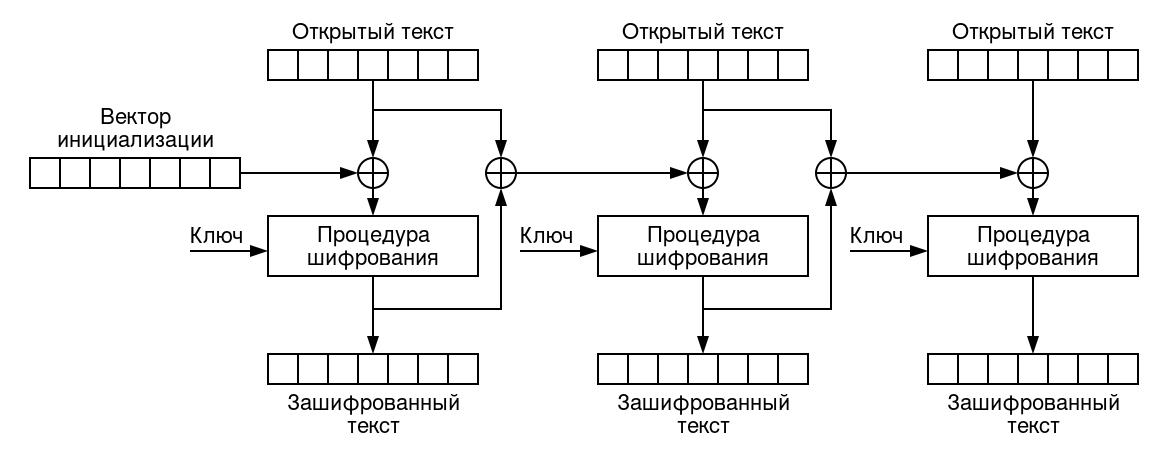
\includegraphics[width=1\linewidth]{assets/images/PCBC_Encryption_ru.png}
	\caption{Схема работы \texttt{PCBC} шифрования}
	\label{fig:pcbc}
\end{figure}

На рисунке \ref{fig:des} приведена схема работы алгоритма \texttt{DES}.

\begin{figure}[ht!]
	\centering
	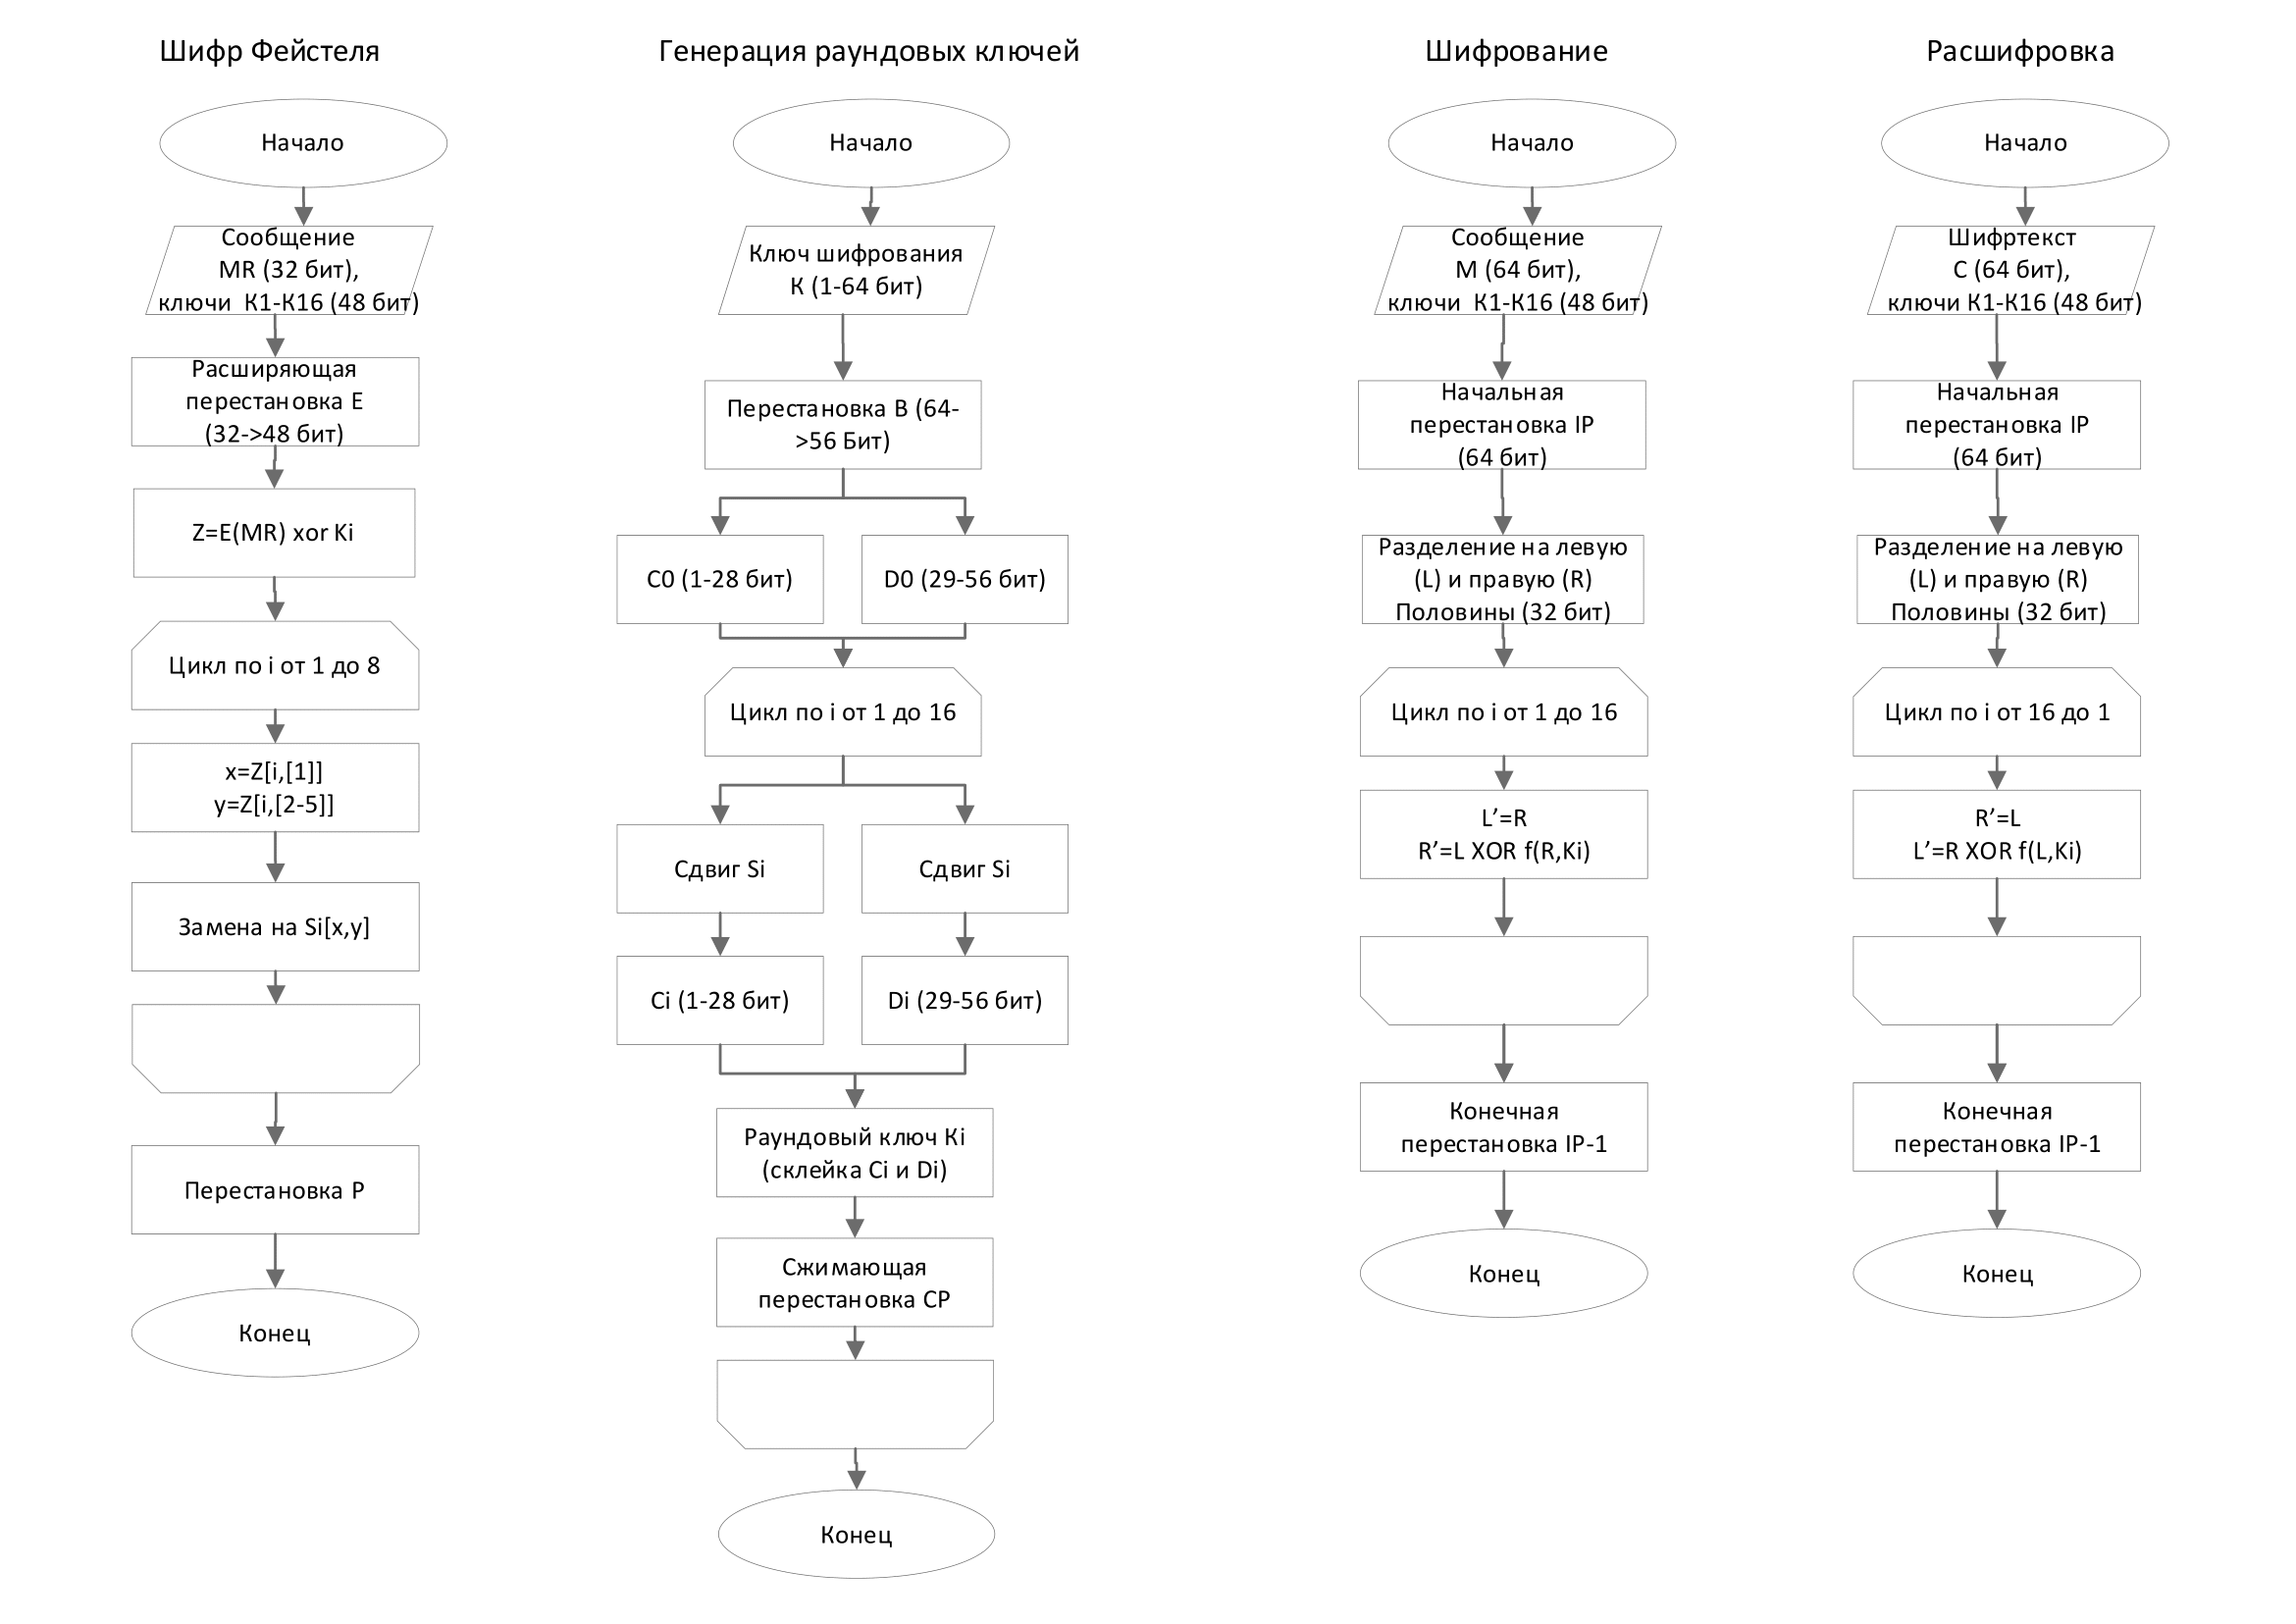
\includegraphics[width=1\linewidth]{assets/images/DES-1.png}
	\caption{Схема работы алгоритма \texttt{DES}}
	\label{fig:des}
\end{figure}

\clearpage

\section{Технологическая часть}

\subsection{Средства реализации}

Для реализации ПО был выбран язык C++~\cite{c++}.
В данном языке есть все требующиеся инструменты для данной лабораторной работы.
В качестве среды разработки была выбрана среда NeoVim~\cite{nvim}.

\subsection{Реализация алгоритма}

\begin{lstinputlisting}[
        caption={\raggedright Реализация алгоритма DES.},
        label={lst:des},
        language={C++},
        linerange={3-32}
    ]{../DES.cpp}
\end{lstinputlisting}

\begin{lstinputlisting}[
        caption={\raggedright Реализация алгоритма DES, часть 2.},
        label={lst:des},
        language={C++},
        linerange={33-66,68-70}
    ]{../DES.cpp}
\end{lstinputlisting}

\begin{lstinputlisting}[
        caption={\raggedright Реализация алгоритма DES, часть 3.},
        label={lst:des-2},
        language={C++},
        linerange={71-81}
    ]{../DES.cpp}
\end{lstinputlisting}

\begin{lstinputlisting}[
        caption={\raggedright Реализация алгоритма шифрования PCBC.},
        label={lst:pcbc},
        language={C++},
        linerange={25-37,39-50}
    ]{../PCBC.cpp}
\end{lstinputlisting}

\subsection{Тестовые данные}

В таблице \ref{tbl:functional_test} приведены тесты, описанные в листинге \ref{lst:tests} для алгоритма \texttt{DES}. 
Применена методология черного ящика. Тесты пройдены \textit{успешно}.
%
\begin{lstinputlisting}[
        caption={\raggedright Реализация функциональных тестов.},
        label={lst:tests},
        language={C++},
        linerange={3-16}
    ]{../tests/des.cpp}
\end{lstinputlisting}

\begin{table}[ht!]
	\begin{center}
		\captionsetup{justification=raggedright,singlelinecheck=off}
		\caption{\label{tbl:functional_test} Функциональные тесты}
		\begin{tabular}{|c|c|c|}
			\hline
			Входная строка & Ключ & Выходная строка \\ 
			\hline
			0000000000000000 & 8000000000000000 & 95A8D72813DAA94D \\
                        EA024714AD5C4D84 & 2BD6459F82C5B300 & 126EFE8ED312190A \\
			F0F0F0F0F0F0F0F0 & F0F0F0F0F0F0F0F0 & 2A2891F65BB8173C \\
                        0011223344556677 & 0001020304050607 & 3EF0A891CF8ED990 \\
      0000000001000000 & 0000000000000000 & 4D49DB1532919C9F \\
                        0000000000000000 & 0000000000000000 & 8CA64DE9C1B123A7 \\
      1414141414141414 & 1414141414141414 & 377B7F7CA3E5BBB3 \\
			\hline
		\end{tabular}
	\end{center}
\end{table}

\clearpage
\section*{\large{ЗАКЛЮЧЕНИЕ}}
В данной лабораторной работе:

\begin{enumerate}
    \item проведен анализ симметричного алгоритма шифрования \texttt{DES} и \texttt{PCBC} режима шифрования;
    \item описаны вышеперечисленные алгоритмы;
    \item релизовано програмное обеспечение с использованием описанных алгоритмов.
\end{enumerate}
